
\documentclass[11pt]{article}
\usepackage{geometry} % see geometry.pdf on how to lay out the page. There's lots.
\geometry{a4paper} % or letter or a5paper or ... etc
\usepackage{amssymb,amsmath}
\usepackage{multirow}
\usepackage{graphicx}
% \geometry{landscape} % rotated page geometry

% See the ``Article customise'' template for come common customisations

\title{}
\author{}
\date{} % delete this line to display the current date

%%% BEGIN DOCUMENT
\begin{document}

\maketitle
\tableofcontents

\section{The Standard Model}
The Standard Model of particle physics was painstakingly constructed over the 20th century and stands as one of the most thoroughly-verified theories in science.  The Standard Model (SM) is a quantum field theory that incorporates two different types of matter particles, the quarks and the leptons, as well as three fundamental forces and their corresponding particles.  However, as we will see, it has several notable shortcomings that attract considerable attention from both theorists and experimentalists.  

\subsection{Quarks and Leptons}
The quarks and the leptons are perhaps the most familiar subatomic particles, as they are the particles that make up matter.  For example, a hydrogen atom is composed of a proton (three quarks) and an electron (a lepton).  There are six quarks total, three ``up-type'' with an electric charge of +2/3 and three ``down-type'' with charge of -1/3.  There are also three leptons, which are electrically charged and massive (the electron, muon and tau), and three neutrinos, which are electrically neutral and nearly massless (the electron, muon and tau neutrinos).  We can classify the quarks and leptons according to ``generation'', where each generation is composed of one up-type quark, one down-type quark, one lepton, and one neutrino.  The quarks and leptons are summarized in Table \ref{tab:QLTable}.

\begin{table}
	\begin{tabular}{| c || c | c | c | c |}
		\multicolumn{3}{c}{Quarks} \\
		\hline
		Generation &  Flavor & Electric Charge & Mass (MeV) & Interactions\\
		\hline
		\multirow{4}{*}{1} & up \it{(u)} & +2/3 \\
		    & down \it{(d)} & -1/3  \\
		    & electron \it{(e)}& -1 \\
		    & electron neutrino \it{($\nu_{e}$)} & 0 \\
		\hline
		\multirow{2}{*}{2} & charm \it{(c)} & +2/3 \\
		    & strange \it{(s)} & -1/3 \\
		    & muon \it{($\mu$)} & -1 \\
		    & muon neutrino \it{($\nu_{\mu}$)} & 0 \\
		\hline 
		\multirow{2}{*}{3} & top \it{(t)} & +2/3 \\
		    & bottom \it{(b)} & -1/3  \\ 
		    & tau \it{($\tau$)} & -1 \\
		    & tau neutrino \it{($\nu_{\tau}$)} & 0 \\		    
		\hline
	\end{tabular}
	\label{tab:QLTable}
\end{table}

All of the quarks and leptons are fermions, meaning they have half-integer spin.

\subsection{Bosons and Forces}

The forces between fermions are carried by bosons, which are integer spin particles.  There are three forces described in the Standard Model: electromagnetic, weak, and strong.  The electromagnetic force is carried by the photon and describes, for example, electric forces between particles.  Photons are massless and as a result, the electromagnetic field can extend infinitely far.  The weak force is carried by W$^+$, W$^-$ and Z$^0$ bosons.  These particles are massive, which means that they are limited in how far they can travel and thus the weak force is confined to distance scales approximately the size of an atomic nucleus.  The weak force is involved when one type of fermion changes into another type of fermion, for example, when a neutron decays or a nucleus fissions.  The strong force is carried by gluons, which are massless but because of confinement, the strong force is restricted to the nuclear scale.  The strong force is responsible for holding quarks together into protons, neutrons and other hadrons. Last, there is the gravitational force, which we will neglect as it is many orders of magnitude weaker than the other forces under discussion.

The electromagnetic and weak forces, as it turns out, can be unified into a single ``electroweak'' force, as discovered in the middle part of the 20th century.  Electroweak unification makes it particularly notable that the weak force vector bosons (W$^+$, W$^-$ and Z$^0$) are heavy, with masses of order 100 GeV, while the photon is massless.  The means by which the vector bosons acquire mass, which is known as electroweak symmetry breaking, happens via the Higgs mechanism.  The Higgs mechanism, and the particle which conveys the Higgs field (the Higgs boson), are explained in more detail in further sections.  Further unification of forces, between the electroweak and strong forces, remains an unfinished project in physics but a topic of much research.  

\section{Electroweak Symmetry Breaking and the Higgs Mechanism}
 
As mentioned above, the Higgs mechanism breaks electroweak symmetry and provides masses to the vector bosons.  

We can start with the Lagrangian

\begin{equation}
L = -(D^\mu \phi) ^\dagger (D_\mu \phi)-\frac{1}{4}F^{\mu \nu}F_{\mu \nu}
\label{EMLagrangian}
\end{equation}

which describes scalar electrodynamics.  We can specify 

\begin{equation}
V(\phi) =  \mu^2(\phi ^\dagger \phi) - \lambda^2 (\phi \phi^\dagger)^2
\label{Vtostart}
\end{equation}

and the observe that the vacuum expectation value (VEV) of the field $\phi$ is not zero, but rather $\langle 0 | \phi | 0 \rangle$ = V.  

 
 \begin{equation}
 \phi ' = (v+\rho (x)) e^{i\chi (x)}
 \end{equation}
 
 after which the potential portion of the Lagrangian above can be rewritten as something.  As this gauge choice breaks the U(1) symmetry, there arises a massless Goldstone boson associated with the $\chi(x)$ field (the boson must be massless because there are no $\chi(x)$-dependent terms in the potential).
 
 
 
\section{Supersymmetry}

\begin{centering}
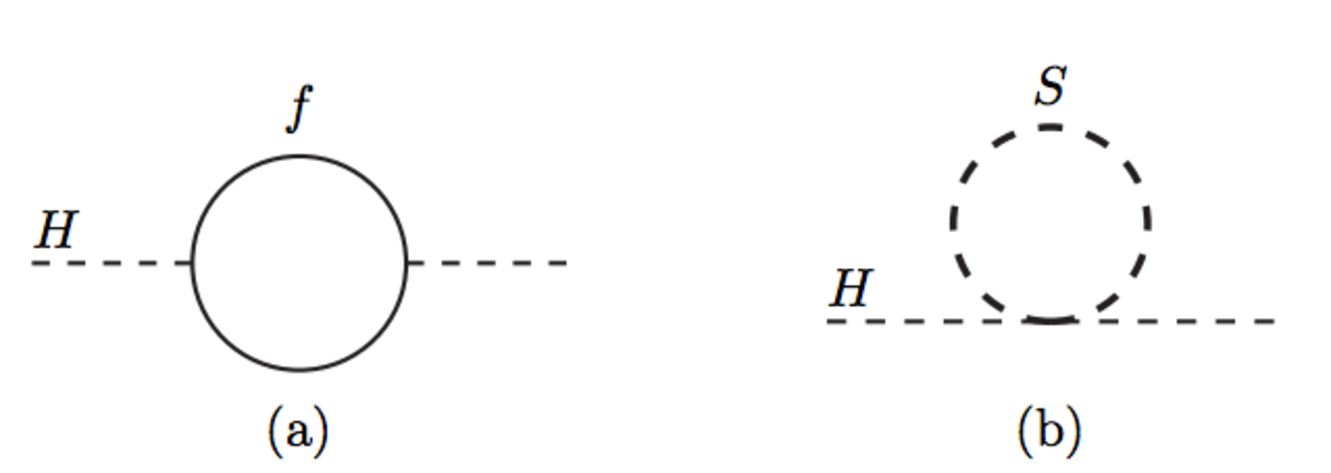
\includegraphics[width=0.6\textwidth]{/Users/caitlinmalone/Documents/Thesis/Theory/FeynmanDiagrams/Higgs_mass_corrections.pdf}\label{fig:higgs_mass_corrections}
\end{centering}

Despite its robustness in the face of experimental scrutiny, the Standard Model has several important shortcomings.  One of the most important is the hierarchy problem, which refers to the quadratic divergence of the Higgs mass via self-coupling.  On the one hand, it is intuitive (and now experimentally verified) that the Higgs mass is of the same order of magnitude as the masses of the vector bosons.  On the other hand, the Higgs can couple to itself via fermion-antifermion pairs, which introduces correction terms to the Higgs mass.  For example, the diagram shown in Figure~\ref{fig:higgs_mass_corrections} (a) contributes the following correction term to the mass:

\begin{equation}
\delta m_H^2 = -\frac{|\lambda_f |^2}{8\pi^2}[\Lambda_{UV}^2+\ldots]
\end{equation}

$\Lambda_{UV}$ is the ultraviolet cutoff scale, the energy at which the Standard Model breaks down and new physics must be enter the picture.  The exact value of $\Lambda_{UV}$ is not known, but a reasonable a priori guess would be the Planck scale, about $10^{19}$ GeV.  However, since the experimentally measured mass of the Higgs is about 125 GeV, there needs to be fine-tuning on the scale of $10^{30}$ GeV for the numbers to come out correctly.

Supersymmetry solves this problem by introducing a mirror set of particles to the Standard Model particles, where each SM boson has a corresponding supersymmetric fermion and each SM fermion has a SUSY boson.  These SUSY particles would also couple to the Higgs, and introduce additional terms to the mass, namely

\begin{equation}
\delta m_H^2 = \frac{|\lambda_s |^2}{16\pi^2}[\Lambda_{UV}^2-2m_2^2ln(\Lambda_{UV}/m_s)+\ldots]
\end{equation}

The ultraviolet cutoff $\Lambda_{UV}$ enters again here, this time with the opposite sign, so that the two terms end up largely canceling when the Higgs mass is computed.  

Another appealing feature of SUSY is that it adjust the coupling constants of the three SM forces.  At very high energies the coupling constants come close to the same value, but do not quite match up, a theoretically unsatisfying fact that SUSY addresses.  When SUSY enters the picture, the running values of the coupling constants change such that they unify at a high energy scale.

\includegraphics[width=\textwidth]{/Users/caitlinmalone/Documents/Thesis/Theory/FeynmanDiagrams/3_couplings.pdf}\label{fig:couplings}

One feature of SUSY is that it's a very unconstrained set of theories--depending on the details of the SUSY version involved, there can be hundreds or thousands (or more) new supersymmetric particles that might enter the pictures.  Similarly, SUSY equations can have many free parameters and it is very difficult, perhaps impossible, to probe all the SUSY phase space.  Phenomenologists address this problem in a number of ways, the most important of which for this thesis is the proposal of the MSSM, or Minimally Supersymmetric Standard Model.  The MSSM makes a number of assumptions about the SUSY parameters and their relationships so as to constrain the number of free parameters to a bare minimum of 19.  

\section{Higgs Physics in Supersymmetry}
Once the constraints of the MSSM have restricted the SUSY phase space to a more tractable 19 parameters, we can see the impact of SUSY on the Higgs sector.  In the MSSM, there is not a single Higgs, but rather a total of 5: three neutral Higgs bosons, called $h^0$, $H^0$, and $A^0$, and two electrically charged bosons $H^+$ and $H^-$.



\end{document}